\chapter{Application's modules}\label{ch:modules}
In this chapter we present briefly the modules that compose our application.
The application is Client-Server, the client has a graphical user interface and
the server is a stateful multi-threaded server which use a Neo4j database for
data persistency.

\section{Client}\label{sec:client}

The client application has been developed using JavaFX for the graphical user
interface. The Views used are organized in Panels, which groups functionalities
for searching Users and Restaurant, a form for User Preferences and Restaurants
creation and modification. Furthermore the Users with administrator
functionalities will have an administration panel where it is possible to add
Cities and Cuisines. Further information on the Client module can be found in
\chref{ch:usermanual}.

\begin{figure}[!h]
	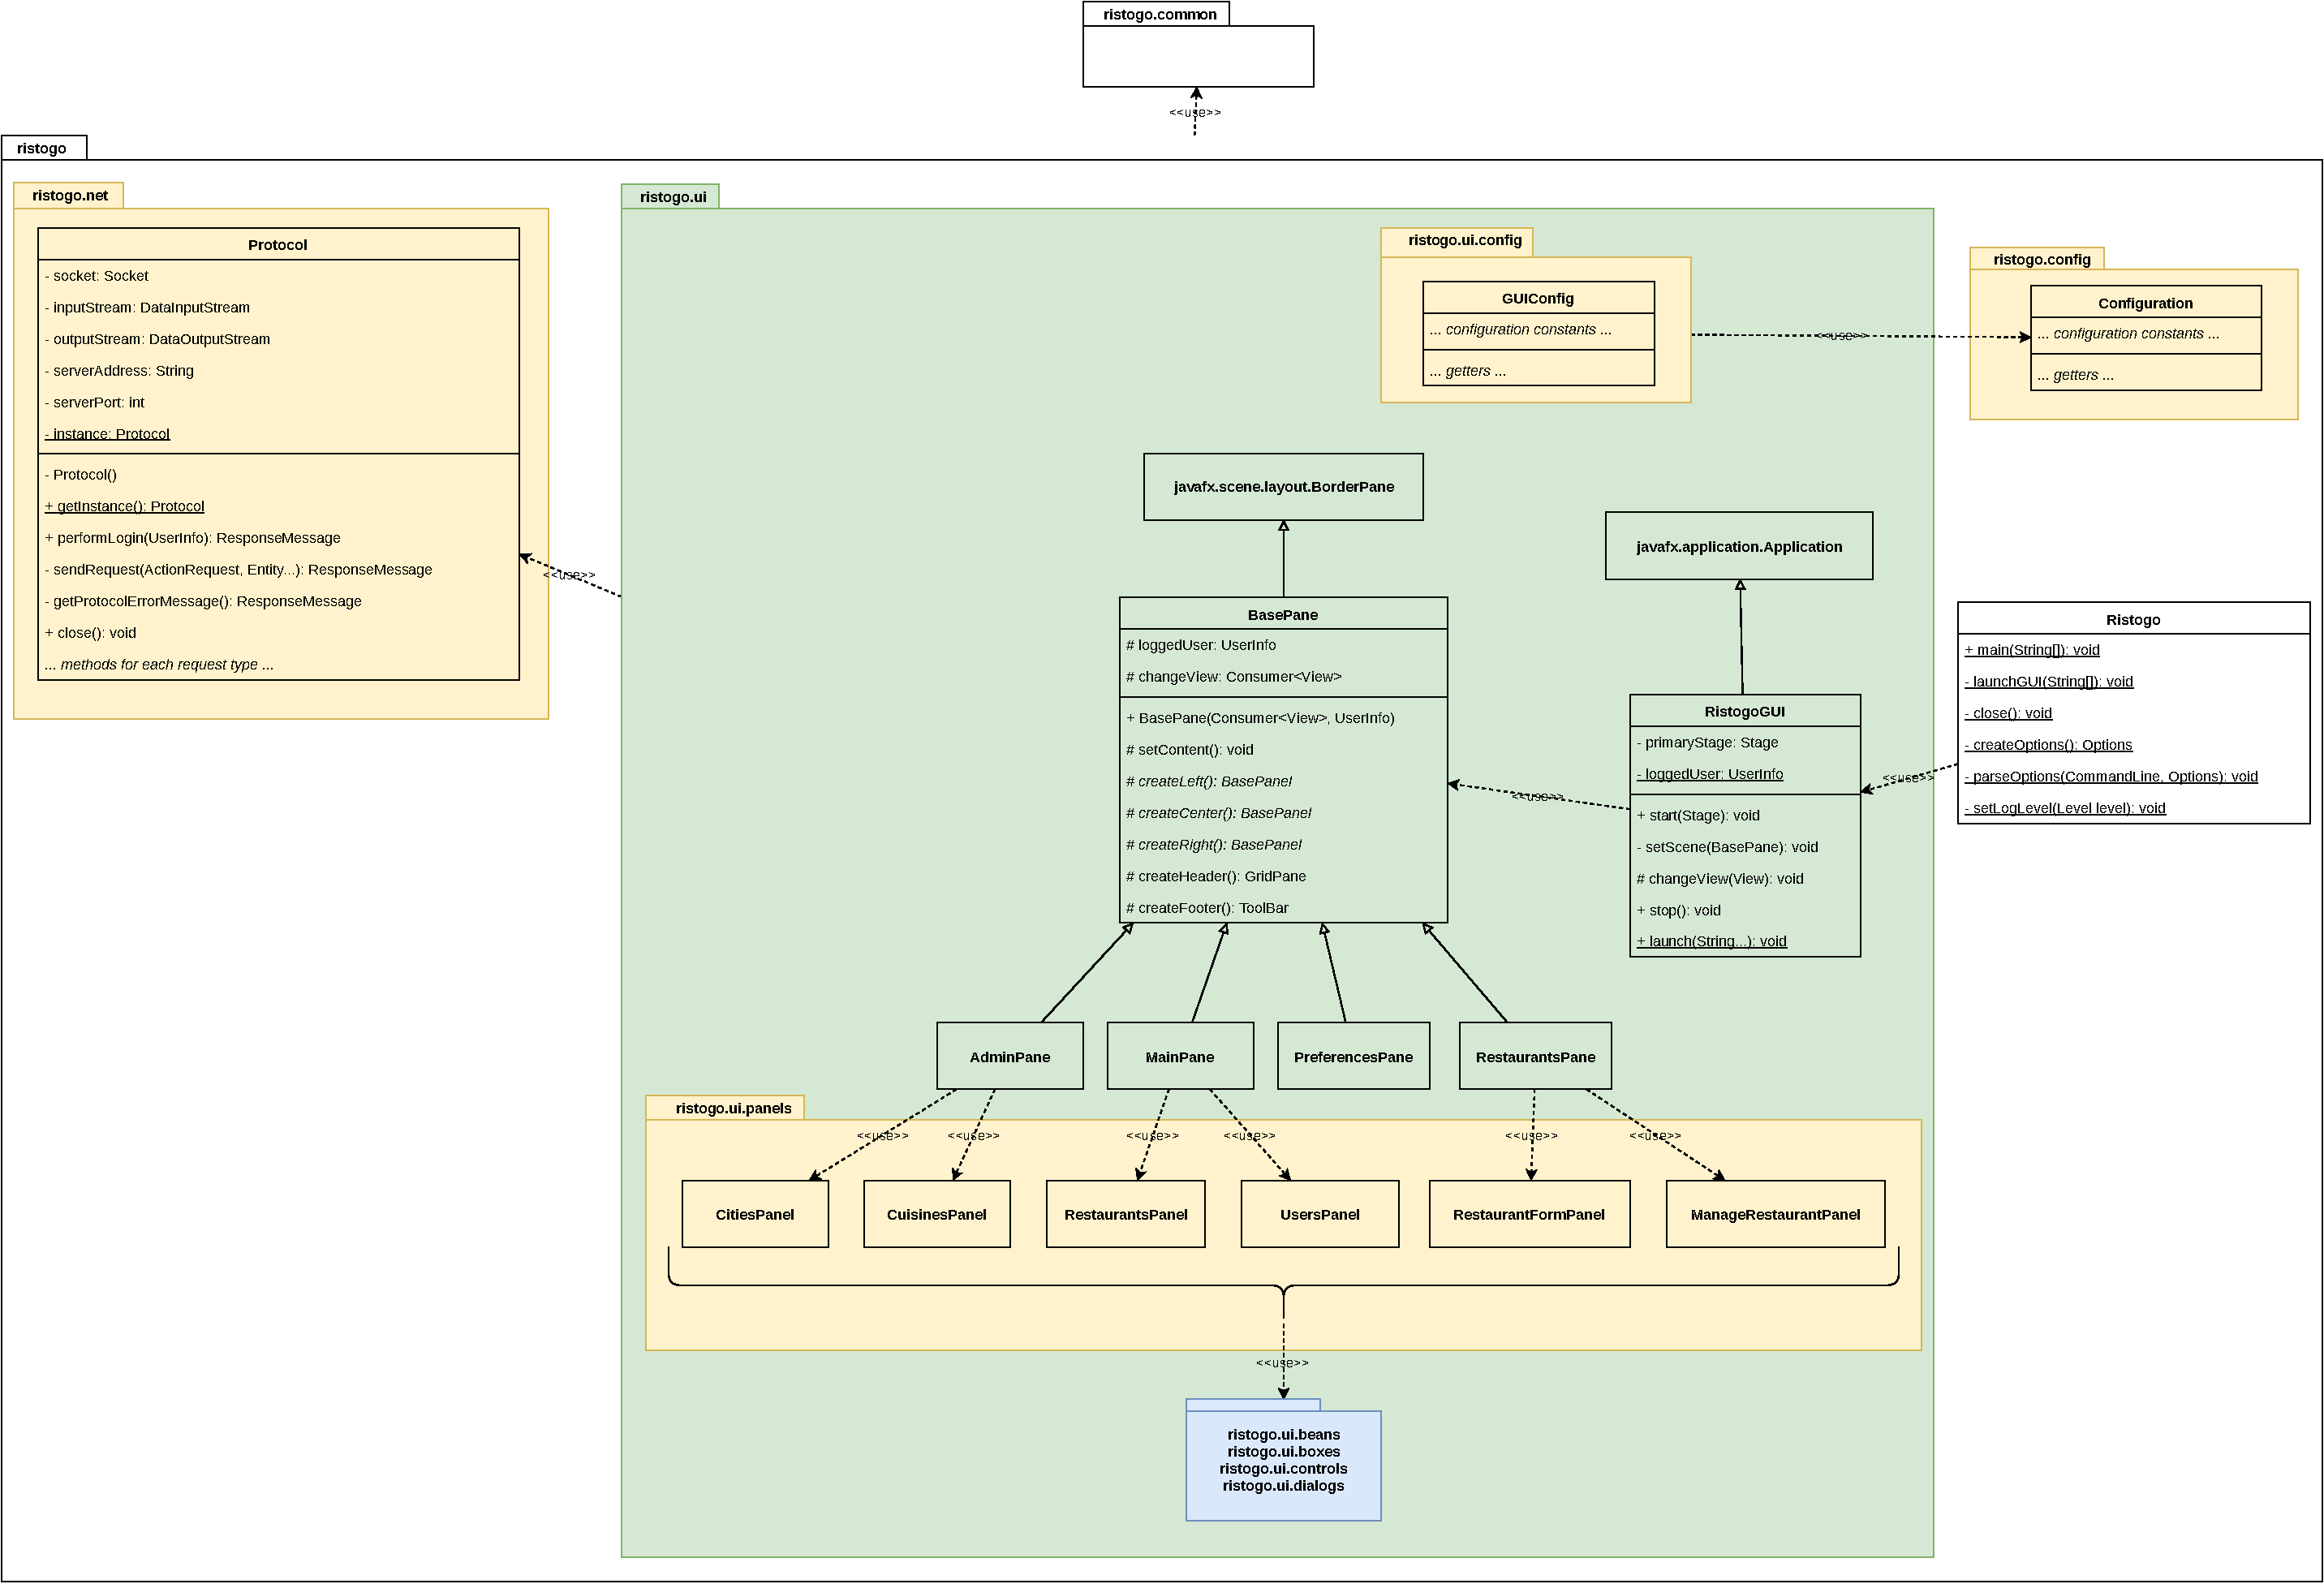
\includegraphics[width=\textwidth]{client}
	\caption{Client UML class diagram.}\label{fig:client}
\end{figure}

\section{Server}\label{sec:server}

The server is a multi-threaded stateful server. The multithreading has been
achieved using a reusable thread pool.

For each user connected the state is maintained on the server for all the
connection time.

The connection with the database use bolt protocol, a Neo4j specific protocol,
which being native is faster and lighter then HTTP based connection. The Data
Access Layer has been designed using a Object Graph Mapping library, thus
allowing us to easily perform CRUD operation on the DB and to implement complex
functionalities using Cypher queries.

To avoid memory exhausting problems the Driver for the database use a pool of
sessions that can be reused among different threads, this has some consequences
from the point of view of the consistency between memory and database, since
some operations may be deferred or done using cached data. Thus to avoid
inconsistency problem every time a request is finished we clear and close the
session so that the driver can recreate a new one, so that the memory can be
freed from cached data and loaded at the next request. In this way  we can be
sure that the data on which we work is completely consistent with the database
and that we have in memory only the data needed for the operation.

\begin{figure}[!h]
	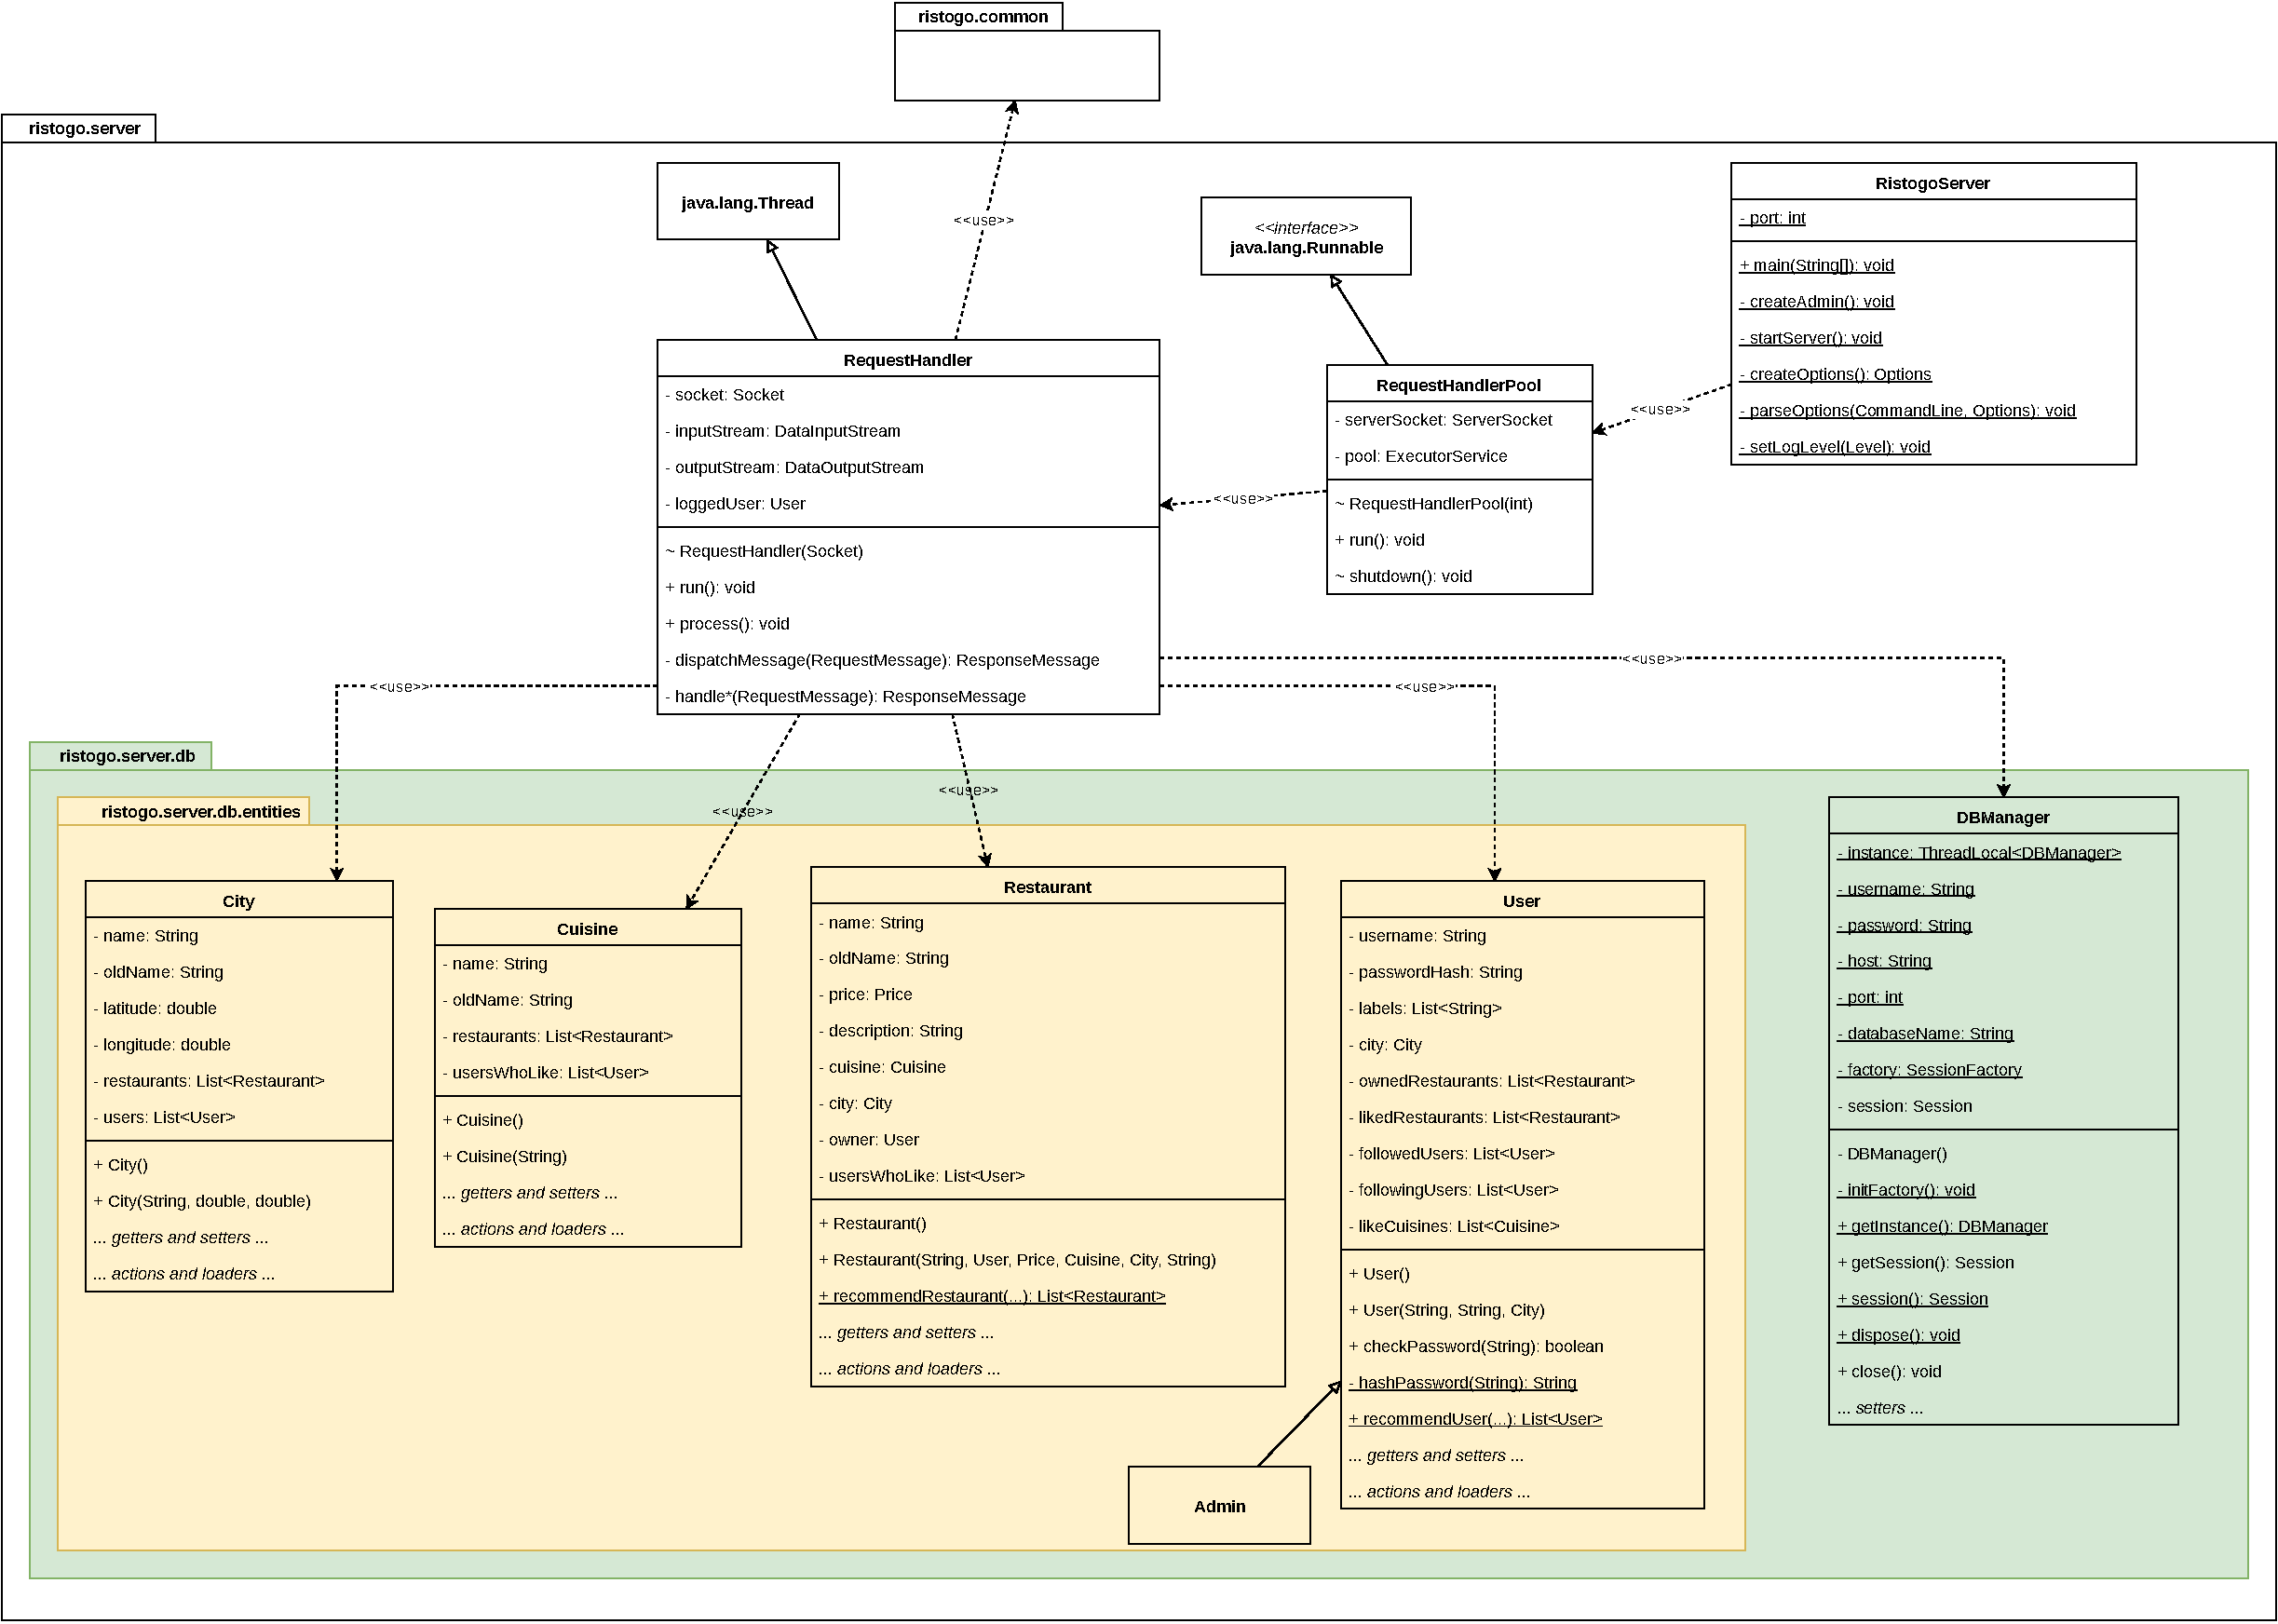
\includegraphics[width=\textwidth]{server}
	\caption{Server UML class diagram.}\label{fig:server}
\end{figure}

\section{Common classes}\label{sec:common}

The common classes are serializable classes that are shared between the
application modules. These classes are used for communication purposes.


\begin{figure}[!h]
	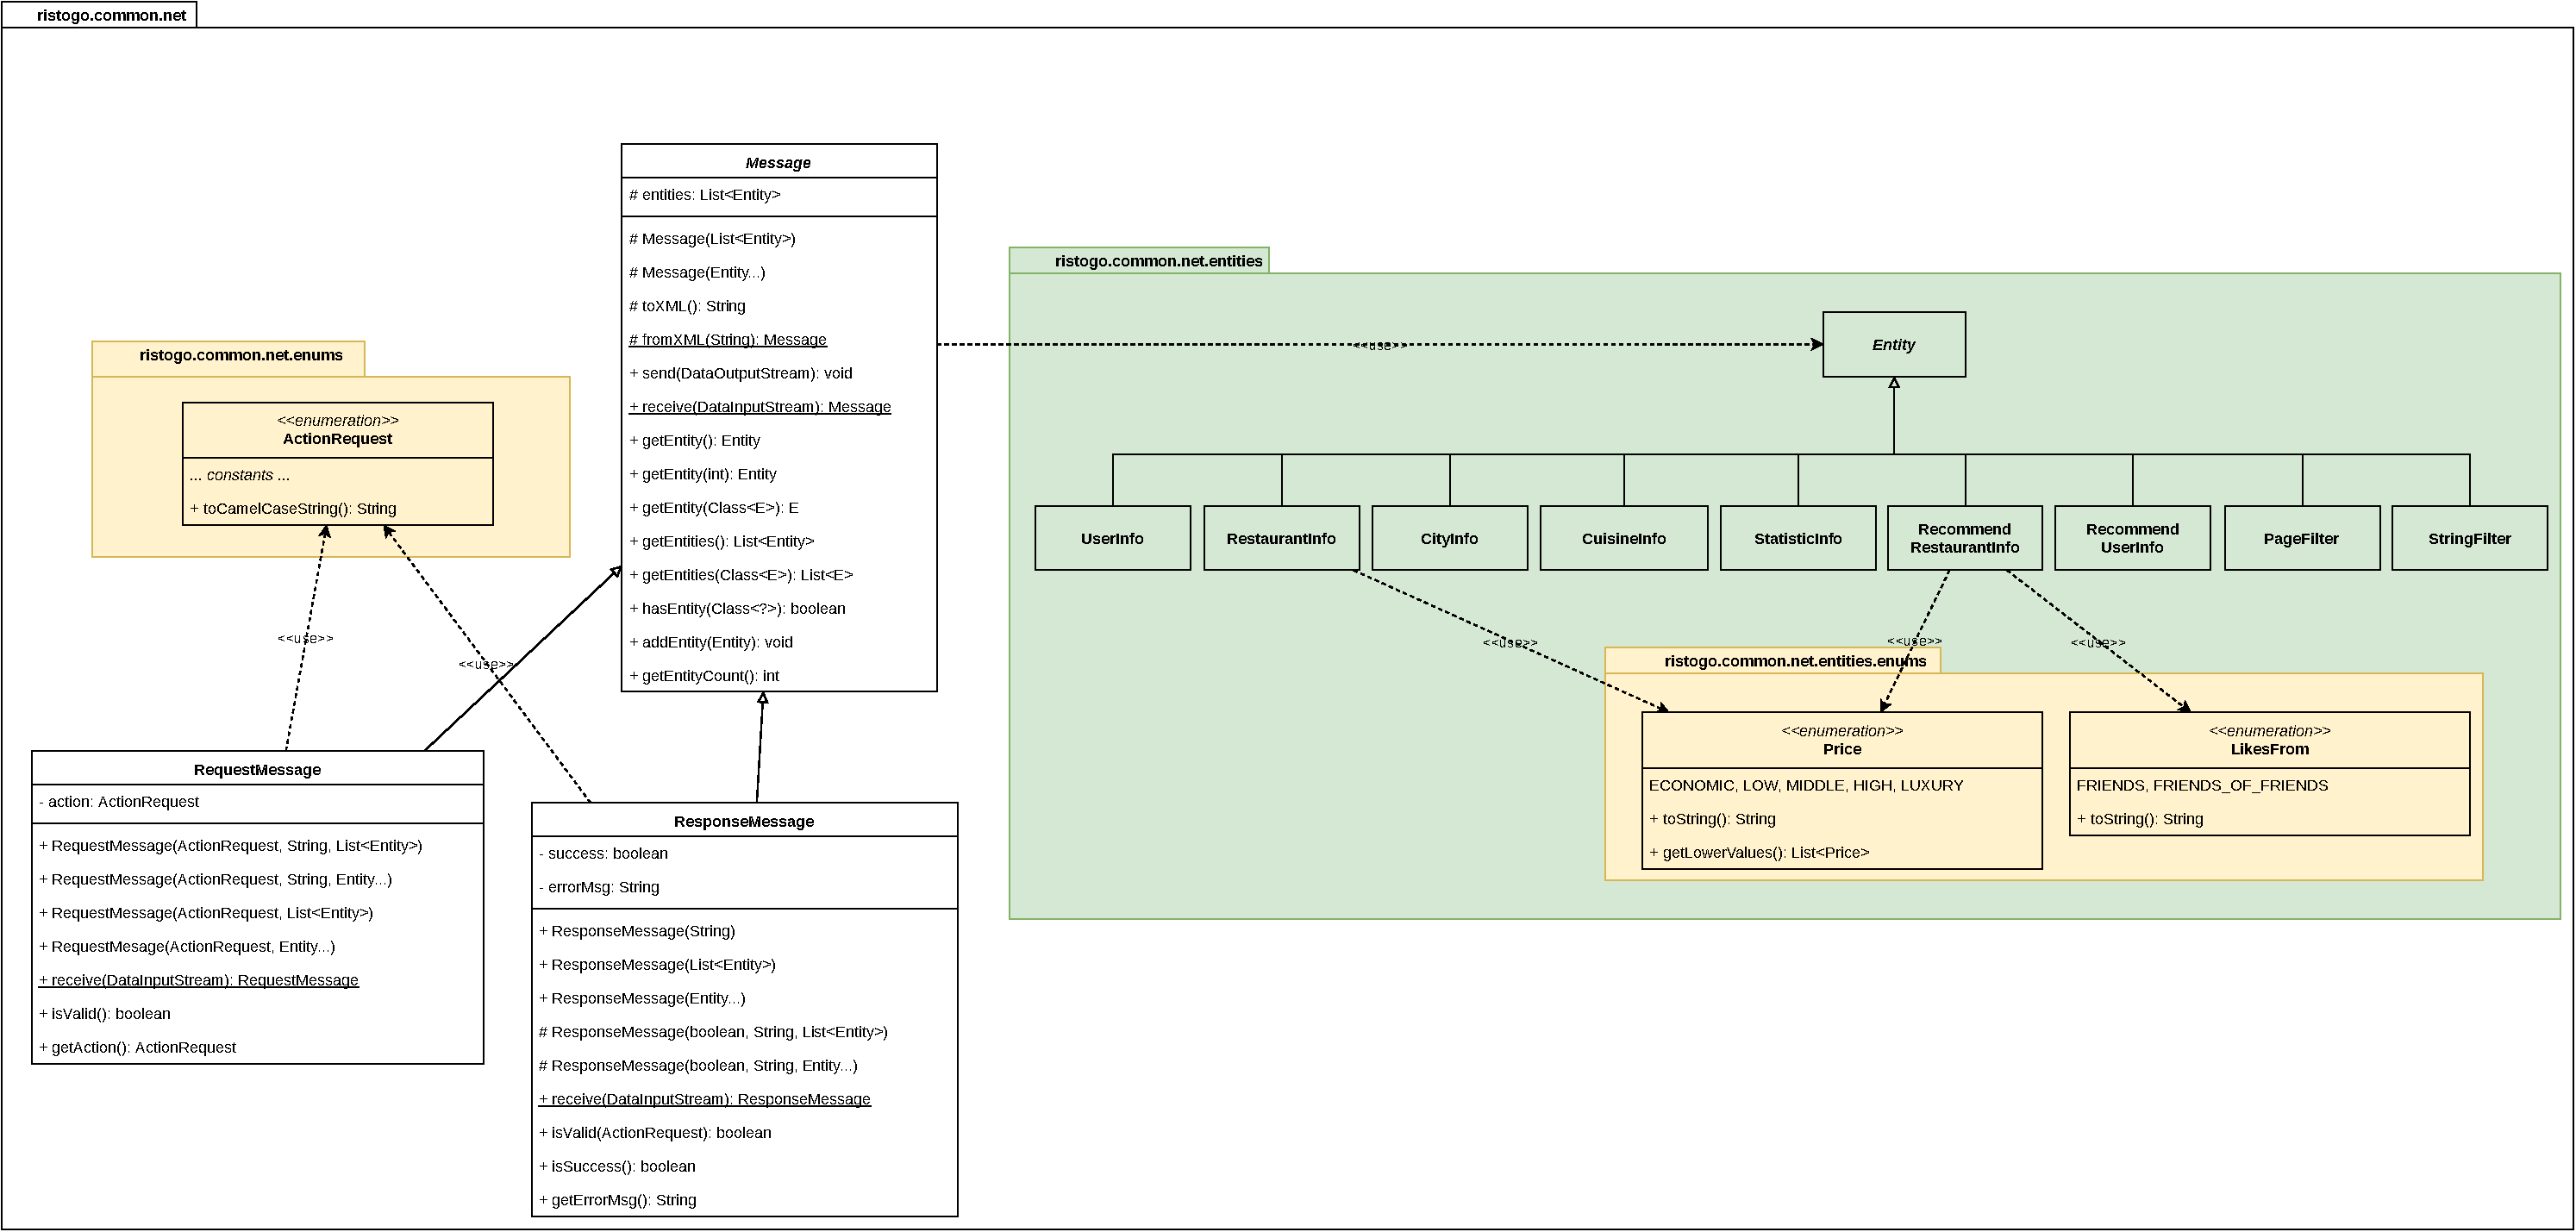
\includegraphics[width=\textwidth]{common}
	\caption{Server UML class diagram.}\label{fig:common}
\end{figure}
